% Options for packages loaded elsewhere
\PassOptionsToPackage{unicode}{hyperref}
\PassOptionsToPackage{hyphens}{url}
%
\documentclass[
]{article}
\usepackage{lmodern}
\usepackage{amssymb,amsmath}
\usepackage{ifxetex,ifluatex}
\ifnum 0\ifxetex 1\fi\ifluatex 1\fi=0 % if pdftex
  \usepackage[T1]{fontenc}
  \usepackage[utf8]{inputenc}
  \usepackage{textcomp} % provide euro and other symbols
\else % if luatex or xetex
  \usepackage{unicode-math}
  \defaultfontfeatures{Scale=MatchLowercase}
  \defaultfontfeatures[\rmfamily]{Ligatures=TeX,Scale=1}
\fi
% Use upquote if available, for straight quotes in verbatim environments
\IfFileExists{upquote.sty}{\usepackage{upquote}}{}
\IfFileExists{microtype.sty}{% use microtype if available
  \usepackage[]{microtype}
  \UseMicrotypeSet[protrusion]{basicmath} % disable protrusion for tt fonts
}{}
\makeatletter
\@ifundefined{KOMAClassName}{% if non-KOMA class
  \IfFileExists{parskip.sty}{%
    \usepackage{parskip}
  }{% else
    \setlength{\parindent}{0pt}
    \setlength{\parskip}{6pt plus 2pt minus 1pt}}
}{% if KOMA class
  \KOMAoptions{parskip=half}}
\makeatother
\usepackage{xcolor}
\IfFileExists{xurl.sty}{\usepackage{xurl}}{} % add URL line breaks if available
\IfFileExists{bookmark.sty}{\usepackage{bookmark}}{\usepackage{hyperref}}
\hypersetup{
  pdftitle={Ejercicio 6},
  hidelinks,
  pdfcreator={LaTeX via pandoc}}
\urlstyle{same} % disable monospaced font for URLs
\usepackage[margin=1in]{geometry}
\usepackage{color}
\usepackage{fancyvrb}
\newcommand{\VerbBar}{|}
\newcommand{\VERB}{\Verb[commandchars=\\\{\}]}
\DefineVerbatimEnvironment{Highlighting}{Verbatim}{commandchars=\\\{\}}
% Add ',fontsize=\small' for more characters per line
\usepackage{framed}
\definecolor{shadecolor}{RGB}{248,248,248}
\newenvironment{Shaded}{\begin{snugshade}}{\end{snugshade}}
\newcommand{\AlertTok}[1]{\textcolor[rgb]{0.94,0.16,0.16}{#1}}
\newcommand{\AnnotationTok}[1]{\textcolor[rgb]{0.56,0.35,0.01}{\textbf{\textit{#1}}}}
\newcommand{\AttributeTok}[1]{\textcolor[rgb]{0.77,0.63,0.00}{#1}}
\newcommand{\BaseNTok}[1]{\textcolor[rgb]{0.00,0.00,0.81}{#1}}
\newcommand{\BuiltInTok}[1]{#1}
\newcommand{\CharTok}[1]{\textcolor[rgb]{0.31,0.60,0.02}{#1}}
\newcommand{\CommentTok}[1]{\textcolor[rgb]{0.56,0.35,0.01}{\textit{#1}}}
\newcommand{\CommentVarTok}[1]{\textcolor[rgb]{0.56,0.35,0.01}{\textbf{\textit{#1}}}}
\newcommand{\ConstantTok}[1]{\textcolor[rgb]{0.00,0.00,0.00}{#1}}
\newcommand{\ControlFlowTok}[1]{\textcolor[rgb]{0.13,0.29,0.53}{\textbf{#1}}}
\newcommand{\DataTypeTok}[1]{\textcolor[rgb]{0.13,0.29,0.53}{#1}}
\newcommand{\DecValTok}[1]{\textcolor[rgb]{0.00,0.00,0.81}{#1}}
\newcommand{\DocumentationTok}[1]{\textcolor[rgb]{0.56,0.35,0.01}{\textbf{\textit{#1}}}}
\newcommand{\ErrorTok}[1]{\textcolor[rgb]{0.64,0.00,0.00}{\textbf{#1}}}
\newcommand{\ExtensionTok}[1]{#1}
\newcommand{\FloatTok}[1]{\textcolor[rgb]{0.00,0.00,0.81}{#1}}
\newcommand{\FunctionTok}[1]{\textcolor[rgb]{0.00,0.00,0.00}{#1}}
\newcommand{\ImportTok}[1]{#1}
\newcommand{\InformationTok}[1]{\textcolor[rgb]{0.56,0.35,0.01}{\textbf{\textit{#1}}}}
\newcommand{\KeywordTok}[1]{\textcolor[rgb]{0.13,0.29,0.53}{\textbf{#1}}}
\newcommand{\NormalTok}[1]{#1}
\newcommand{\OperatorTok}[1]{\textcolor[rgb]{0.81,0.36,0.00}{\textbf{#1}}}
\newcommand{\OtherTok}[1]{\textcolor[rgb]{0.56,0.35,0.01}{#1}}
\newcommand{\PreprocessorTok}[1]{\textcolor[rgb]{0.56,0.35,0.01}{\textit{#1}}}
\newcommand{\RegionMarkerTok}[1]{#1}
\newcommand{\SpecialCharTok}[1]{\textcolor[rgb]{0.00,0.00,0.00}{#1}}
\newcommand{\SpecialStringTok}[1]{\textcolor[rgb]{0.31,0.60,0.02}{#1}}
\newcommand{\StringTok}[1]{\textcolor[rgb]{0.31,0.60,0.02}{#1}}
\newcommand{\VariableTok}[1]{\textcolor[rgb]{0.00,0.00,0.00}{#1}}
\newcommand{\VerbatimStringTok}[1]{\textcolor[rgb]{0.31,0.60,0.02}{#1}}
\newcommand{\WarningTok}[1]{\textcolor[rgb]{0.56,0.35,0.01}{\textbf{\textit{#1}}}}
\usepackage{graphicx,grffile}
\makeatletter
\def\maxwidth{\ifdim\Gin@nat@width>\linewidth\linewidth\else\Gin@nat@width\fi}
\def\maxheight{\ifdim\Gin@nat@height>\textheight\textheight\else\Gin@nat@height\fi}
\makeatother
% Scale images if necessary, so that they will not overflow the page
% margins by default, and it is still possible to overwrite the defaults
% using explicit options in \includegraphics[width, height, ...]{}
\setkeys{Gin}{width=\maxwidth,height=\maxheight,keepaspectratio}
% Set default figure placement to htbp
\makeatletter
\def\fps@figure{htbp}
\makeatother
\setlength{\emergencystretch}{3em} % prevent overfull lines
\providecommand{\tightlist}{%
  \setlength{\itemsep}{0pt}\setlength{\parskip}{0pt}}
\setcounter{secnumdepth}{-\maxdimen} % remove section numbering
\usepackage{float}
\usepackage{booktabs}
\usepackage{longtable}
\usepackage{array}
\usepackage{multirow}
\usepackage{wrapfig}
\usepackage{colortbl}
\usepackage{pdflscape}
\usepackage{tabu}
\usepackage{threeparttable}
\usepackage{threeparttablex}
\usepackage[normalem]{ulem}
\usepackage{makecell}
\usepackage{xcolor}

\title{Ejercicio 6}
\author{}
\date{\vspace{-2.5em}}

\begin{document}
\maketitle

\hypertarget{librerias}{%
\subsection{Librerias}\label{librerias}}

\begin{Shaded}
\begin{Highlighting}[]
\KeywordTok{library}\NormalTok{(cluster)}
\KeywordTok{library}\NormalTok{(FactoMineR)}
\KeywordTok{library}\NormalTok{(ggrepel)}
\KeywordTok{library}\NormalTok{(kableExtra)}
\KeywordTok{library}\NormalTok{(tidyverse)}
\KeywordTok{source}\NormalTok{(here}\OperatorTok{::}\KeywordTok{here}\NormalTok{(}\StringTok{"src"}\NormalTok{, }\StringTok{"utils.R"}\NormalTok{))}
\end{Highlighting}
\end{Shaded}

\begin{verbatim}
Para cada configuracion medida en los pepinillos (cualitativa, cuantitativa y
molecular) obtenemos la matriz de distancia entre los puntos en el
plano principal y calculamos la correlacion entre pares de matrices.
\end{verbatim}

\begin{Shaded}
\begin{Highlighting}[]
\NormalTok{conc_}\DecValTok{2}\NormalTok{_}\DecValTok{3}\NormalTok{ <-}\StringTok{ }\KeywordTok{cor}\NormalTok{(datos_}\DecValTok{2}\NormalTok{_dist, datos_}\DecValTok{3}\NormalTok{_dist)}\OperatorTok
\StringTok{             }\KeywordTok{round}\NormalTok{(}\DecValTok{2}\NormalTok{)}

\NormalTok{conc_}\DecValTok{2}\NormalTok{_}\DecValTok{5}\NormalTok{ <-}\StringTok{ }\KeywordTok{cor}\NormalTok{(datos_}\DecValTok{2}\NormalTok{_dist, datos_}\DecValTok{5}\NormalTok{_dist)}\OperatorTok
\StringTok{            }\KeywordTok{round}\NormalTok{(}\DecValTok{2}\NormalTok{)}

\NormalTok{conc_}\DecValTok{3}\NormalTok{_}\DecValTok{5}\NormalTok{ <-}\StringTok{ }\KeywordTok{cor}\NormalTok{(datos_}\DecValTok{3}\NormalTok{_dist, datos_}\DecValTok{5}\NormalTok{_dist)}\OperatorTok
\StringTok{             }\KeywordTok{round}\NormalTok{(}\DecValTok{2}\NormalTok{)}
\end{Highlighting}
\end{Shaded}

\begin{verbatim}
Al obtener las correlacion entre las matrices de distancias de las diferentes
caracterizaciones sobre el plano principal, observamos que la correlacion mas
baja se obtiene al comparar la caracterizacion cuantitativa con la molecular,
siendo de 0.6. Este resultado no es para nada desalentador, por el
contrario, nos indica que al incorporar una nueva dimension (caracteristicas
moleculares) sobre la informacion cuantitativa que ya conociamos
estamos adquiriendo nueva informacion, permitiendo explicar de una mejor forma el
comportamiento y caracterizacion de los pepinillos. 
Luego, la correlacion entre las matrices de distancias de las caracterizaciones 
cualitativa y molecular es de 0.67, indicando de esta forma una concordancia
media-alta.
La correlacion entre las matrices de distancias de las caracterizaciones 
cualitativa y cuantitativa en el plano principal es de
0.78, lo cual nos indica una concordancia alta entre estas caracterizaciones.
\end{verbatim}

\begin{enumerate}
\def\labelenumi{\Alph{enumi})}
\item
  Mida la concordancia entre la caracterización agronómica (cualitativa
  + cuantitativa) y molecular (planos principales)
\item
  Con APG halle el consenso entre las configuraciones (plano principal)
  obtenidas en base a datos cualitativos, cuantitativos y moleculares.
\end{enumerate}

\begin{Shaded}
\begin{Highlighting}[]
\NormalTok{df =}\StringTok{ }\KeywordTok{cbind}\NormalTok{(}
\NormalTok{  datos_}\DecValTok{2}\NormalTok{,}
\NormalTok{  datos_}\DecValTok{3}\NormalTok{,}
\NormalTok{  datos_}\DecValTok{5}
\NormalTok{) }\OperatorTok
\StringTok{  }\KeywordTok{as.data.frame}\NormalTok{()}\OperatorTok
\StringTok{  }\KeywordTok{round}\NormalTok{(}\DecValTok{2}\NormalTok{)}

\KeywordTok{colnames}\NormalTok{(df) =}\StringTok{ }\KeywordTok{c}\NormalTok{(}\StringTok{"C1"}\NormalTok{, }\StringTok{"C2"}\NormalTok{, }\StringTok{"Q1"}\NormalTok{, }\StringTok{"Q2"}\NormalTok{, }\StringTok{"M1"}\NormalTok{, }\StringTok{"M2"}\NormalTok{)}

\NormalTok{gpa <-}\StringTok{ }\KeywordTok{GPA}\NormalTok{(}
\NormalTok{  df, }
  \DataTypeTok{group =} \KeywordTok{c}\NormalTok{(}\DecValTok{2}\NormalTok{, }\DecValTok{2}\NormalTok{, }\DecValTok{2}\NormalTok{), }
  \DataTypeTok{name.group =} \KeywordTok{c}\NormalTok{(}\StringTok{"Cuantiativa"}\NormalTok{, }\StringTok{"Cualitativa"}\NormalTok{, }\StringTok{"Molecular"}\NormalTok{),}
  \DataTypeTok{graph =} \OtherTok{TRUE}\NormalTok{, }
  \DataTypeTok{axes =} \KeywordTok{c}\NormalTok{(}\DecValTok{1}\NormalTok{,}\DecValTok{2}\NormalTok{)}
\NormalTok{)}
\end{Highlighting}
\end{Shaded}

\begin{center}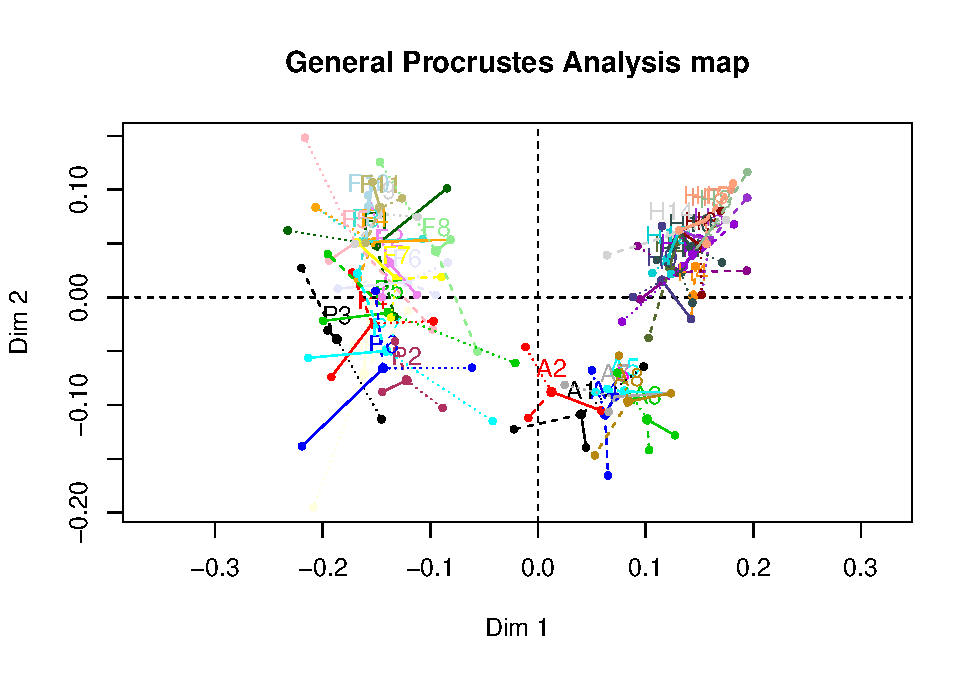
\includegraphics{parte_6_files/figure-latex/unnamed-chunk-5-1} \end{center}

\begin{enumerate}
\def\labelenumi{\Alph{enumi})}
\tightlist
\item
  Identifique si hay algún tipo de pepino para el cual hay más
  discrepancia entre estas tres caracterizaciones
\end{enumerate}

\begin{Shaded}
\begin{Highlighting}[]
\NormalTok{df <-}\StringTok{ }\KeywordTok{as.data.frame}\NormalTok{(}\KeywordTok{head}\NormalTok{(gpa}\OperatorTok{$}\NormalTok{PANOVA}\OperatorTok{$}\NormalTok{objet, }\DecValTok{-1}\NormalTok{))}
\NormalTok{df}\OperatorTok{$}\NormalTok{tipo <-}\StringTok{ }\KeywordTok{substr}\NormalTok{(}\KeywordTok{rownames}\NormalTok{(df), }\DecValTok{1}\NormalTok{, }\DecValTok{1}\NormalTok{)}

\NormalTok{df }\OperatorTok\StringTok{ }
\StringTok{    }\KeywordTok{group_by}\NormalTok{(tipo) }\OperatorTok
\StringTok{    }\KeywordTok{summarise}\NormalTok{(}\DataTypeTok{media =} \KeywordTok{mean}\NormalTok{(SSresidual)) }\OperatorTok
\StringTok{    }\KeywordTok{arrange}\NormalTok{(}\KeywordTok{desc}\NormalTok{(media))}\OperatorTok
\StringTok{    }\KeywordTok{kable}\NormalTok{() }\OperatorTok\StringTok{ }
\StringTok{    }\KeywordTok{kable_styling}\NormalTok{(}\DataTypeTok{font_size =} \DecValTok{12}\NormalTok{) }\OperatorTok\StringTok{ }
\StringTok{    }\KeywordTok{kable_classic_2}\NormalTok{() }
\end{Highlighting}
\end{Shaded}

\begin{table}
\centering\begingroup\fontsize{12}{14}\selectfont

\begin{tabular}{l|r}
\hline
tipo & media\\
\hline
P & 0.6074664\\
\hline
F & 0.3259472\\
\hline
A & 0.1929178\\
\hline
H & 0.1458124\\
\hline
\end{tabular}
\endgroup{}
\end{table}

\begin{verbatim}
Para identificar si hay algun tipo de pepino que tiene mas discrepancia entre
las caracteristicas cualitativas, cuantitativas y moleculares se calculan la sumas de
cuadrados residuales promedio para cada una de las variedades. Como podemos observar, 
los pepinos tipo .... tienen 
\end{verbatim}

\textbf{E.} Finalice el análisis con un cluster UPGMA obtenido a partir
de la configuración de consenso

\begin{Shaded}
\begin{Highlighting}[]
\NormalTok{dist<-}\KeywordTok{dist}\NormalTok{(df, }\DataTypeTok{method =} \StringTok{"euclidean"}\NormalTok{)}
\NormalTok{cluster_upgma<-}\KeywordTok{hclust}\NormalTok{( dist, }\DataTypeTok{method =} \StringTok{"average"}\NormalTok{)}
\NormalTok{cluster_upgma_data<-}\StringTok{ }\KeywordTok{dendro_data_k}\NormalTok{(cluster_upgma, }\DataTypeTok{k=}\DecValTok{4}\NormalTok{)}

\KeywordTok{ggplot}\NormalTok{(cluster_upgma_data}\OperatorTok{$}\NormalTok{segments) }\OperatorTok{+}\StringTok{ }
\StringTok{  }\KeywordTok{geom_segment}\NormalTok{(}
    \KeywordTok{aes}\NormalTok{(}\DataTypeTok{x =}\NormalTok{ x, }\DataTypeTok{y =}\NormalTok{ y, }\DataTypeTok{xend =}\NormalTok{ xend, }\DataTypeTok{yend =}\NormalTok{ yend, }\DataTypeTok{color =} \KeywordTok{as.factor}\NormalTok{(clust)),}
    \DataTypeTok{size =} \FloatTok{1.2}\NormalTok{,}
    \DataTypeTok{lineend =} \StringTok{"round"}
\NormalTok{  ) }\OperatorTok{+}\StringTok{ }
\StringTok{  }\KeywordTok{geom_text}\NormalTok{(}
    \KeywordTok{aes}\NormalTok{(}\DataTypeTok{x =}\NormalTok{ x, }\DataTypeTok{y =}\NormalTok{ y }\OperatorTok{-}\StringTok{ }\FloatTok{0.40}\NormalTok{, }\DataTypeTok{label =}\NormalTok{ label, }\DataTypeTok{color =} \KeywordTok{as.factor}\NormalTok{(clust)), }
    \DataTypeTok{data =}\NormalTok{ cluster_upgma_data}\OperatorTok{$}\NormalTok{labels}
\NormalTok{  ) }\OperatorTok{+}\StringTok{ }
\StringTok{  }\KeywordTok{coord_flip}\NormalTok{() }\OperatorTok{+}\StringTok{ }
\StringTok{  }\KeywordTok{labs}\NormalTok{(}
    \DataTypeTok{y =} \StringTok{"Distancia"}
\NormalTok{  ) }\OperatorTok{+}\StringTok{ }
\StringTok{  }\KeywordTok{scale_colour_manual}\NormalTok{(}
    \DataTypeTok{values =} \KeywordTok{c}\NormalTok{(}\StringTok{"grey30"}\NormalTok{, scales}\OperatorTok{::}\KeywordTok{hue_pal}\NormalTok{()(}\DecValTok{4}\NormalTok{))}
\NormalTok{  ) }\OperatorTok{+}\StringTok{ }
\StringTok{  }\KeywordTok{theme}\NormalTok{(}
    \DataTypeTok{panel.grid.major =} \KeywordTok{element_blank}\NormalTok{(), }
    \DataTypeTok{panel.grid.minor =} \KeywordTok{element_blank}\NormalTok{(), }
    \DataTypeTok{panel.background =} \KeywordTok{element_blank}\NormalTok{(),}
    \DataTypeTok{axis.title.x =} \KeywordTok{element_text}\NormalTok{(}\DataTypeTok{size =} \DecValTok{14}\NormalTok{), }
    \DataTypeTok{axis.title.y =} \KeywordTok{element_blank}\NormalTok{(), }
    \DataTypeTok{axis.text.x =} \KeywordTok{element_text}\NormalTok{(}\DataTypeTok{size =} \DecValTok{12}\NormalTok{),}
    \DataTypeTok{axis.text.y =} \KeywordTok{element_blank}\NormalTok{(), }
    \DataTypeTok{axis.line =} \KeywordTok{element_blank}\NormalTok{(), }
    \DataTypeTok{axis.ticks.y =} \KeywordTok{element_blank}\NormalTok{(),}
    \DataTypeTok{plot.title =} \KeywordTok{element_text}\NormalTok{(}\DataTypeTok{hjust =} \FloatTok{0.5}\NormalTok{),}
    \DataTypeTok{legend.position =} \StringTok{"none"}
\NormalTok{  )}
\end{Highlighting}
\end{Shaded}

\begin{center}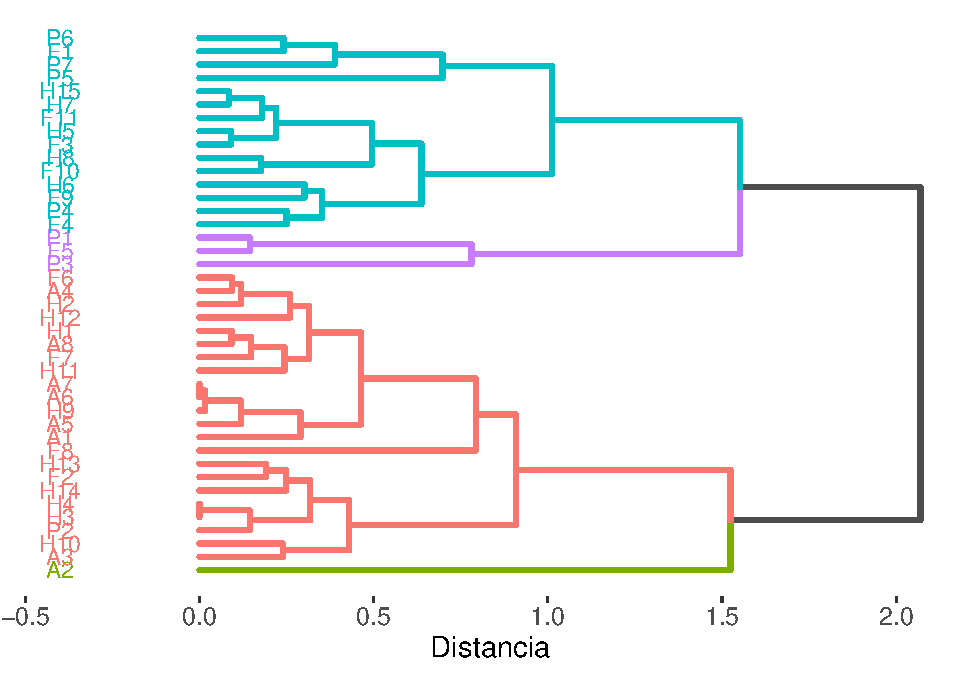
\includegraphics{parte_6_files/figure-latex/unnamed-chunk-7-1} \end{center}

\end{document}
